\documentclass[12pt]{article}
\usepackage[left=0.9in, right=0.9in, top=1in, bottom=1in]{geometry}
\usepackage{tikz}
\usepackage{setspace}
\usepackage{hyperref}
\usepackage{amsfonts, amssymb, amsmath} 
\usepackage{titlesec}
\usepackage{pgfplots}
\pgfplotsset{compat=newest}
\usepackage{graphicx}
\usepackage{wrapfig}
\usepackage{caption}
\usepackage{enumitem}
\usetikzlibrary{shadows.blur}
\usepackage{lmodern}
\setlength{\parskip}{0pt}
\setlength{\parindent}{0pt}

\title{\textcolor{purple}{\Huge\textbf{Analízis IV}}}
\author{1. gyakorlat}
\date{Szabó Krisztián}

\renewcommand{\contentsname}{Tartalom}
\newcommand{\R}{\mathbb{R}}
\newcommand{\N}{\mathbb{N}}
\newcommand{\E}{\exists}
\newcommand{\mm}{\mathbf{m}}
\newcommand{\MM}{\mathbf{M}}
\newcommand{\K}{\mathbb{K}}
\newcommand{\D}{\mathcal{D}_f}

\definecolor{modernyellow}{HTML}{F4E4BC}
\definecolor{moderngreen}{HTML}{BDDCBD}

\tikzset
{
	definition/.style={
		draw,
		fill=modernyellow,
		line width=1pt,
		rounded corners,
		drop shadow={shadow blur steps=5,shadow xshift=1ex,shadow yshift=-1ex},
		text width=0.9\textwidth,
		inner sep=10pt
	},
	theorem/.style={
		draw,
		fill=moderngreen,
		line width=1pt,
		rounded corners,
		drop shadow={shadow blur steps=5,shadow xshift=1ex,shadow yshift=-1ex},
		text width=0.9\textwidth,
		inner sep=10pt
	},
	proof/.style={
		fill=white,
		rectangle,
		drop shadow={shadow blur steps=5,shadow xshift=1ex,shadow yshift=-1ex, moderngreen},
		text width=0.9\textwidth,
		inner sep=6pt,
	},
	proof1/.style={
		fill=white,
		rectangle,
		drop shadow={shadow blur steps=5,shadow xshift=1ex,shadow yshift=0, moderngreen},
		text width=0.9\textwidth,
		inner sep=6pt,
	}
}

\begin{document}
    \maketitle
    \tableofcontents
    \newpage
    \section{Feladat}
    Hengerkoordinátákra áttérve számítsuk ki az alábbi integrált:
    \[
        \int\int\int_H (x^2 + y^2) \, dx \, dy \, dz,
    \]
    ahol $H$ az alábbi egyenletű felületek által határolt korlátos és zárt térrész:
    \[
        x^2 + y^2 = 2z, \quad \wedge \quad z = 2.
    \]

    Vizsgáljuk meg a $H$ halmazt geometriailag:
    \[
        z = \frac{x^2 + y^2}{2}
    \]

    Ha a $z = 2$ sík berajzolásra kerülne, akkor az alábbi korlátos és zárt térrészt kapjuk:
    \[
        H := \left\{ \left(x, \, y, \, \frac{x^2 + y^2}{2} \right) \in \R^3 : \frac{x^2 + y^2}{2} \leq 2 \right\}.
    \]
    Ahhoz, hogy hengertranszformációt alkalmazzunk, induljunk ki a következő ötletből: a $z$ értékek fussák be a $[0, \, 2]$ intervallumot, majd minden $z$ pontnál kapjuk az alábbi körlapot:
    \[
        x^2 + y^2 \leq \left( \sqrt{2z} \right)^2.
    \]
    Ezekből az információkból rakjuk össze a következő transzformációt:
    \[
        H \ni    
        \begin{pmatrix}
            x \\
            y \\
            z
        \end{pmatrix}
        \sim
        \Phi(r, \, \varphi, \, z) :=
        \begin{pmatrix}
            r \cdot \cos(\varphi) \\
            r \cdot \sin(\varphi) \\
            z
        \end{pmatrix}
        \quad \left(z \in [0, \, 2], \, \varphi \in [0, \, 2\pi], \, r \in [0, \, \sqrt{2z}]\right).
    \]
    Az integráltranszformáció tétele alapján az eredeti integál a következő alakot ölti:
    \[
        \int\limits_0^2 \int\limits_0^{\sqrt{2z}} \int\limits_0^{2\pi} r^2 \cdot r \, d\varphi \, dr \, dz
    \].

    \newpage
    \section{Feladat}
    Határozzuk meg az alábbi $K$ kúptest \textit{tehetetlenségi nyomatékát} a $z$ illetve az $x$ tengelyre nézve, ha a kitöltő anyag sűrűsége minden pontban egyenesen arányos az origótól mért távolság négyzetével:
    \[
        K := \left\{ (x, \, y, \, z) \in \R^3 : 0 \leq \frac{1}{2} \cdot \sqrt{y^2 + z^2} \leq x \leq 1 \right\}.
    \]
    
    \newpage
    \section{Feladat}
    Számítsuk ki annak a korlátos és zárt térbeli $T$ testnek a \textit{térfogatát, tömegét} és a $z$-tengelyre vonatkozó \textit{tehetetlenségi nyomatékát}, amelyet az alábbi egyenlőtlenségek definiálnak:
    \[
        \sqrt{x^2 + y^2} \leq z \wedge x^2 + y^2 + z^2 \leq 1,
    \]
    illetve a kitöltő anyag pontonkénti sűrűsége egyenesen arányos az origótól mért távolsággal.

    %\begin{center}
    %    \begin{tikzpicture}
    %        \begin{axis}[
    %            clip=false,
    %            colormap/viridis,
    %            xlabel={$x$}, ylabel={$y$}, zlabel={$z$}
    %        ]
    %      
    %        \addplot3[
    %          surf,
    %          opacity=0.6,
    %          samples=20, domain=0:2*pi, y domain=0:1,
    %          z buffer=sort,
    %        ]
    %        (
    %          {y*cos(deg(x))}, % x-coordinate (parametrized)
    %          {y*sin(deg(x))}, % y-coordinate (parametrized)
    %          {y}              % z-coordinate (y = sqrt(x^2 + y^2))
    %        );
    %      
    %        % Plot the sphere: x^2 + y^2 + z^2 <= 1
    %        \addplot3[
    %          surf,
    %          opacity=0.6,
    %          samples=30, domain=0:360, y domain=0:45,
    %          z buffer=sort,
    %        ]
    %        (
    %          {sin(y)*cos(x)}, % x-coordinate
    %          {sin(y)*sin(x)}, % y-coordinate
    %          {cos(y)}         % z-coordinate
    %        );
    %      
    %        \end{axis}
    %      \end{tikzpicture}
    %\end{center}

    Jelöljük az alábbi ponthalmazokat, az alábbi módon:
    \[
        K := \{ (x, \, y, \, z) \in \R^3 : \sqrt{x^2 + y^2} \leq z \},
    \]
    \[
        G := \{ (x, \, y, \, z) \in \R^3 : x^2 + y^2 + z^2 \leq 1 \}.
    \]

    A $K$ halmaz egy kúptest, míg a $G$ halmaz egy egységsugarú gömböt jelöl. Mi a következő ponthalmaz térfogatát keressük:
    \[
        V := K \cap G.
    \]

    A $V$ halmaz meghatározott térfogatot két részre bontjuk, egy csonkakúpra és egy gömbszeletre. A csonkakúp térfogatát hengerkoordináta transzformációval az alábbi módon számolhatjuk:

    \[
    \Phi(r, \, \varphi, \, z) :=
    \begin{pmatrix}
        r \cdot \cos(\varphi) \\
        r \cdot \sin(\varphi) \\
        z
    \end{pmatrix},
    \]
    ahol
    \[
        z \in [0, \, \sqrt{2} / 2], \, \varphi \in [0, \, 2 \pi], \, r \in [0, \, z].
    \]
    Tehát
    \[
        V(V_1) := \int\limits_0^{\sqrt{2}/2}\int\limits_0^{2\pi}\int\limits_0^z 1 \cdot r \, dr \, d\varphi \, dz.
    \]

    A gömbszelet térfogatát térbeli polárkoordináta transzformációval lehet számolni az alábbi módon:

    \begin{center}
        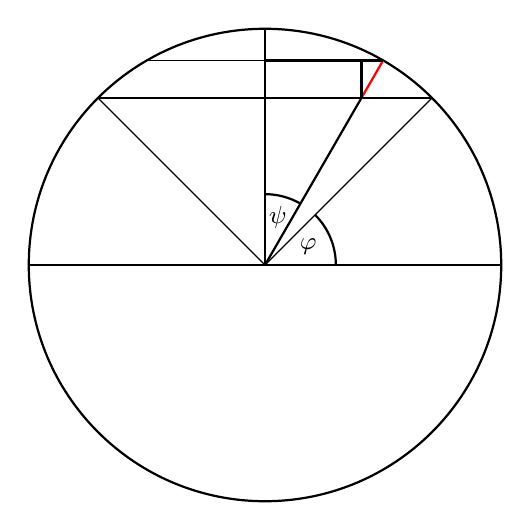
\begin{tikzpicture}[scale=3]
            
            \draw[thick] (0,0) circle [radius=1];
            \draw (-0.70710678118, 0.70710678118) -- (0.70710678118, 0.70710678118);
            \draw (-1, 0) -- (1, 0);
            \draw (0, 0) -- (0, 1);
            \draw (0,0) -- (0.70710678118, 0.70710678118);
            \draw (0,0) -- (-0.70710678118, 0.70710678118);
            
            \draw[thick] (0.3,0) arc[start angle=0, end angle=45, radius=0.3cm];
            \draw[draw=none] (0.20,0) arc[start angle=0, end angle=23.5, radius=0.20cm] node {\small$\varphi$};

            \draw[thick] (0.15,0.25980762113) arc[start angle=60, end angle=90, radius=0.3cm];
            \draw[draw=none] (0.15*0.7,0.25980762113*0.7) arc[start angle=60, end angle=75, radius=0.21cm] node {\small$\psi$};
            
            \draw[thick, red] (0.4082,0.7071) -- (0.5, 0.86602540378);
            \draw[thick] (0, 0) -- (0.4082,0.7071);

            \draw[thick] (0,0.866) -- (0.5, 0.866);
            \draw (-0.5, 0.866) -- (0, 0.866);
            \draw[thick] (0,0) -- (0, 0.866);

            \draw[thick] (0.4082,0.7071) -- (0.4082, 0.866);
            
        \end{tikzpicture}    
    \end{center}
    
    A fenti ábrán két háromszög vastagon kiemelve hasonlók. Mi az piros szakasz hosszát keressük, hogy az alábbi térbeli polárkoordináta transzformációt el tudjuk végezni. Jelöljük a piros szakasz hosszát $\ell$-lel.

    \[
        \Phi(r, \, \varphi, \, \psi) :=
        \begin{pmatrix}
            r \cdot \cos(\varphi) \cdot \sin(\psi) \\
            r \cdot \sin(\varphi) \cdot \sin(\psi) \\
            r \cdot \cos(\psi)
        \end{pmatrix}
    \]
    ahol
    \[
        \varphi \in [0, \, 2 \pi], \, \psi \in [0, \, \pi / 4], \, r \in [1 - \ell, \, 1].
    \]
    Mivel tudjuk, hogy $\varphi = \pi / 4$ és a gömbünk (körünk) sugara $1$, ezért könnyedén kapjuk az alábbi egyenlőséget:
    \[
        \ell = 1 - \frac{\sqrt{2}}{2 \cdot \cos(\psi)}.
    \]
    Így, a maradék gömbszelet térfogata az alábbi transzformációval kiszámolható:
    \[
        V(V_2) := \int\limits_0^{2\pi} \int\limits_0^{\pi / 4} \int\limits_{\frac{\sqrt{2}}{2\cdot \cos(\psi)}}^1 1 \cdot (-r^2) \cdot \sin(\psi) \, dr \, d\psi \, d\varphi.
    \]

    Így kapjuk, hogy a $V = K \cap G$ ponthalmaz térfogata $V_1 + V_2$.

\end{document}